\section{Results}

\paragraph{\textit{NOTE}: For the simulation, we use 0.2 hour as the timestep value, if not mentioned}

\drawBorder

\begin{enumerate}

    \item
        With Position $x_1 = 0\hat{i} + 0\hat{j}$, $x_2 = 1000\hat{i} + 0\hat{j}$ in \si{\km} and velocity $v_1 = 0\hat{i} + 0\hat{j}$, $v_2 = 60\hat{i} + 60\hat{j}$ in \si{\km \per \sec} and equal masses of mass $1e26$ kg

        \begin{figure}[h!]
            \centering
            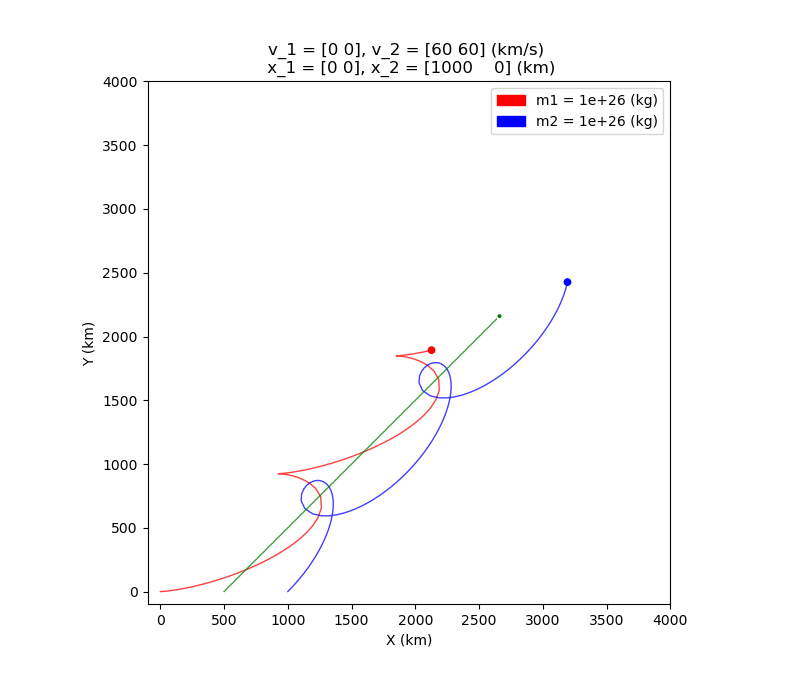
\includegraphics[width=0.8\textwidth]{fig1.png}
        \end{figure}

        This is the plot of the two body system as seen in a non-inertial frame of reference. \\The \textbf{green line} represents the center of mass of the system.

        \newpage

\drawBorder

    \item

        With Position $x_1 = 0\hat{i} + 0\hat{j}$, $x_2 = 3000\hat{i} + 0\hat{j}$ in km and velocity $v_1 = 10\hat{i} + 20\hat{j}$, $v_2 = 0\hat{i} + 40\hat{j}$ in \si{\km \per \sec} and equal masses of mass $1e26$ kg

        \begin{figure}[h!]
            \centering
            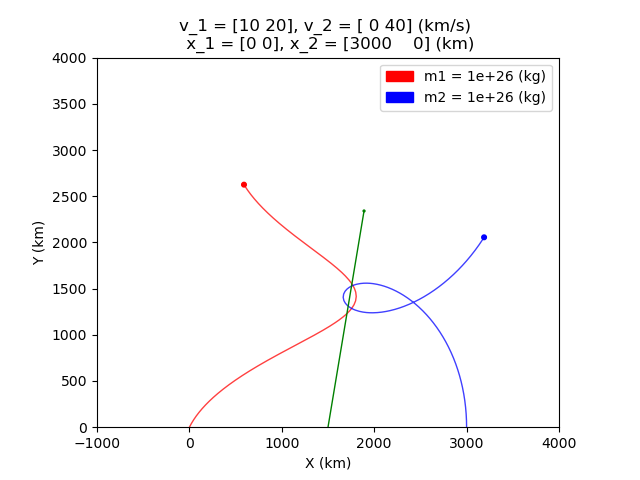
\includegraphics[width=0.8\textwidth]{fig5.png}
        \end{figure}

        Using the \textbf{Algorithm 2.2} mentioned in \textcite{orbital_mechanics_4ed} we can plot the motion of the body relative to another. The below plot shows the relative motion of $m_1$ with respect to $m_2$ using the same initial condition.

        \begin{figure}[h!]
            \centering
            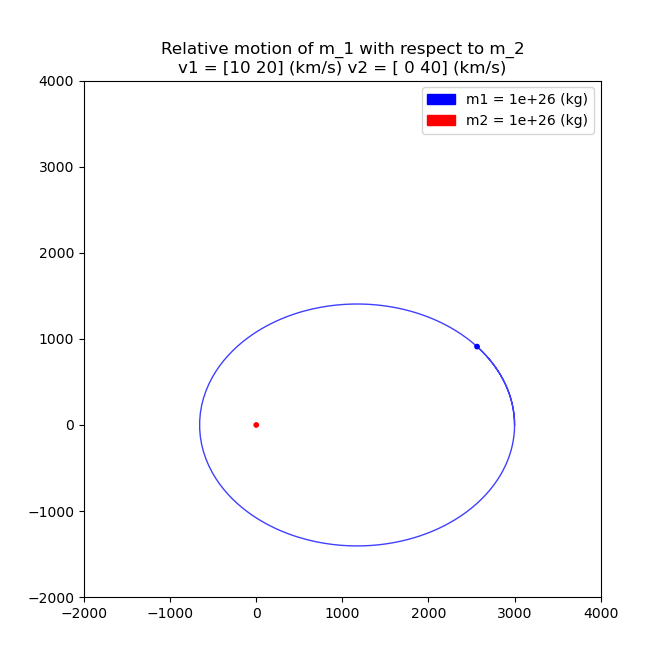
\includegraphics[width=0.7\textwidth]{fig6.png}
        \end{figure}

        \newpage

\drawBorder

    \item
        With Position $x_1 = 500\hat{i} + 100\hat{j}$, $x_2 = 100\hat{i} + 1000\hat{j}$ in km and velocity $v_1 = 10\hat{i} + 10\hat{j}$, $v_2 = -70\hat{i} + 10\hat{j}$ in \si{\km \per \sec} and equal masses of mass $1e26$ kg

        \begin{figure}[h!]
            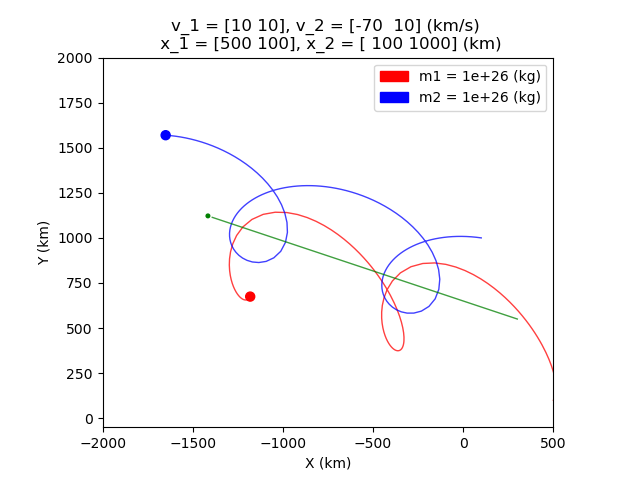
\includegraphics[width=0.8\textwidth]{fig2.png}
            \centering
        \end{figure}

        And motion of $m_1$ relative to $m_2$,

        \begin{figure}[h!]
            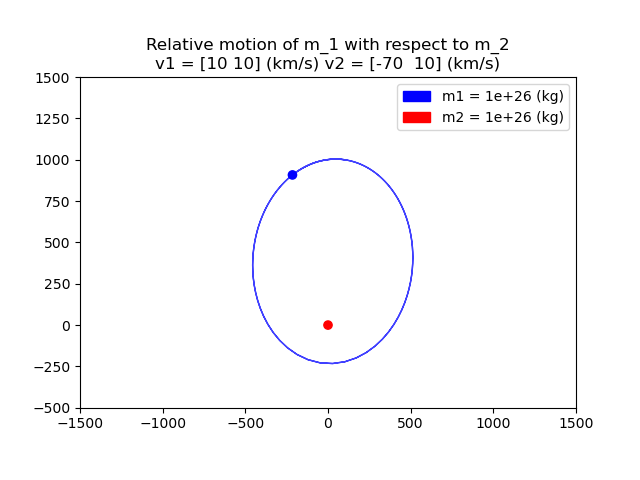
\includegraphics[width=0.8\textwidth]{fig7.png}
            \centering
        \end{figure}


        \newpage

\drawBorder

    \item
        With Position $x_1 = 0\hat{i} + 0\hat{j}$, $x_2 = 1000\hat{i} + 1000\hat{j}$ in \si{\km} and velocity $v_1 = 0\hat{i} + 0\hat{j}$, $v_2 = -30\hat{i} + 10\hat{j}$ \si{\km \per \sec} and masses $m_1 = 1e26$ kg and $m_2 = 1e23$ kg

        \begin{figure}[h!]
            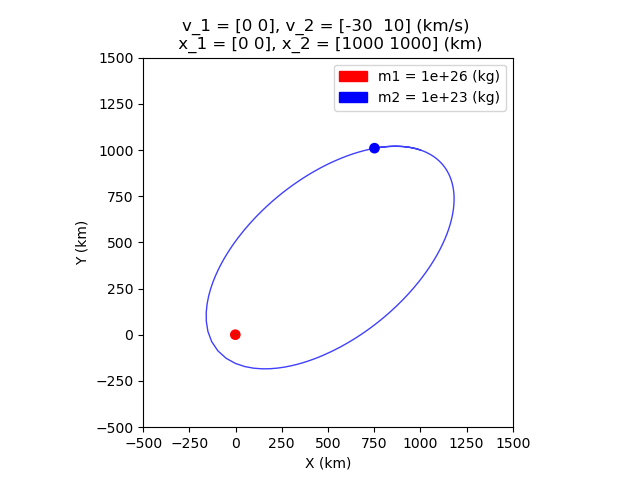
\includegraphics[width=0.8\textwidth]{fig3.png}
            \centering
        \end{figure}

        These conditions allow for a stable orbit of mass $m_2$ around $m_1$ shown in the above plot.

\end{enumerate}
